\chapter{実験2 : 病理画像データセットを用いた実験}
\section{概要}
MNISTの実験から、提案したクエリ選考基準は、既存手法よりもCNNにとって識別率向上に寄与するサンプルを選択できていることが確認できた。
本章では、本研究で提案するシステムを用いて実際に病理画像データセットに対して行った実験について説明する。

\section{実験設定}
\subsection{データセットについて}
本実験では、Camelyon Grand Challenge\cite{Camelyon17}にて公開されたCamelyonデータセットを利用した。
Camelyonデータセットは1000枚のWSIからなり、乳癌のリンパ節転移を自動で検出する識別器を生成することを目的としたデータセットである\todo{図}。
各WSIは一枚あたり100,000×100,000ピクセルの大きさで、細胞組織を含む画像パッチは約10,000から400,000枚になる。
また、それら全ての画像パッチに対して癌か正常かの二値のラベルが付与されている。
ここでも、MNISTで行った実験と同様に各画像パッチのラベルは、クエリとして問い合わせない限り与えられない状況とする。

\section{予備実験}
\todo{都合の良い特徴量とか識別器を使ってるのずるいのかな。他のデータセットでやるべき??}

\subsection{クラスタリング手法の比較}
第3章で述べたクラスタリングに使用する特徴量を比較するために、それぞれの特徴量を用いて病理画像データセットをK-meansによってクラスタリングを行った際の
各クラスター内のラベルの不純度を平均を計算した。不純度が小さいほどクラスター内でのばらつきが小さく良い特徴量だと言える\todo{ちょいあやしいか}。
データセットは100,000枚の病理画像からなり、癌と正常の割合は均等に調整した。
使用したデータセットの詳細は第5章で説明する。
表\ref{table:compare_feat}に示すように、CNNを用いたテクスチャ特徴量であるCompact Bilinear Poolingをクラスタリングに用いるのが妥当であると考えられる。

\begin{table}[h]
  \caption{\label{table:compare_feat}比較実験の結果}
  \center
  \begin{tabular}{c|c} \hline
     手法 & Inpurity \\ \hline
    LBP & 0.396 \\
    CNNの中間特徴量 & 0.335  \\ 
    Compact Bilinear Pooling & $\textbf{0.330}$ \\ \hline
  \end{tabular}
\end{table}

\subsection{線形識別器との比較}
線形識別器はくそだよという話

\section{実験の詳細}
識別機に用いるCNNはGoogLeNetを採用した。他の一般画像認識で利用されるCNNのアーキテクチャの中でも比較的計量で、
医療画像解析ではしばしば用いられるモデルであることから選択した。
少ないラベルで高精度を達成するために、ImageNetのpretrained-modelを初期値として、fine-tuningによって学習を行う。

訓練時に使用するWSIから全ての画像パッチを抽出すると約5,000,000枚に登る。これをラベルなしデータセット$\mathcal{U}$とし、
各クエリ問い合わせでは$\mathcal{U}$からサンプリングされた$\mathcal{U}_i$から選択する。
$\mathcal{U}_i$のサイズは50,000に設定した。

本実験でも、同一クエリ内での情報の重複を避けるためクラスタリングを行う。
予備実験より、クラスタリングに使用する特徴量はCompact Bilinear Poolingを用いたテクスチャ特徴量を採用する。
committeeサイズは10, k-meansのクラスター数$K$は1000、一度に選択するクエリ$\mathcal{Q}$のサイズは100に設定した。
本実験では、実用的な状況に近づけるため、Mnistでの実験のように各iterationでの学習回数を固定にせず
与えられた比較的小さいバリデーションセットの性能が変化しなくなるまで学習を続ける、という設定にした。
バリデーションセットのサイズは100とした。
また、クラスターの代表サンプルから無作為にサンプリングされた100個のサンプルにラベルを付与して学習初期のラベルつきデータとして実験を開始した。
各クエリ問い合わせ毎に10000枚のテストデータに対する識別精度を計測し、ラベルを付与されたデータが10000に到達するまで実験を続けた。
比較手法は、以下の3つを使用した。
\begin{itemize}
  \item Random Sampling
  \item QBDP+Uncertain Sampling
  \item QBDP+Uncertain Sampling+Aug
\end{itemize}
実験ごとのばらつきを考慮し、同一の実験を3回行いその平均と標準偏差を計算した。

\section{実験結果}
本項では上記で述べた実験の結果を示す。
クエリ選考基準として提案手法、比較手法それぞれを使用した際の、ラベル付きサンプル数の増加に対するテスト精度の変化のグラフを図\ref{fig:camelyon_acc_graph}に示す。
Mnistでの実験とは異なり、pretrained-modelからのfine-tuningを行っているため収束早いことがわかる。
ここでも、
これは上記に述べた通り多層ニューラルネットワークが正しくモデルの不確かさを表現できていないからだと推測される。
さらに、推論時にもData Augmentationを利用することで、さらに少ないラベルで高精度を達成していることがわかる。
また、ラベル付きデータセットが1000枚の際に、各手法によってクエリとして選択されたサンプルを図\ref{figure:camelyon_query_examples}に示す。

\begin{figure}[tbp]
    \label{fig:camelyon_acc_graph}
     \begin{center}
      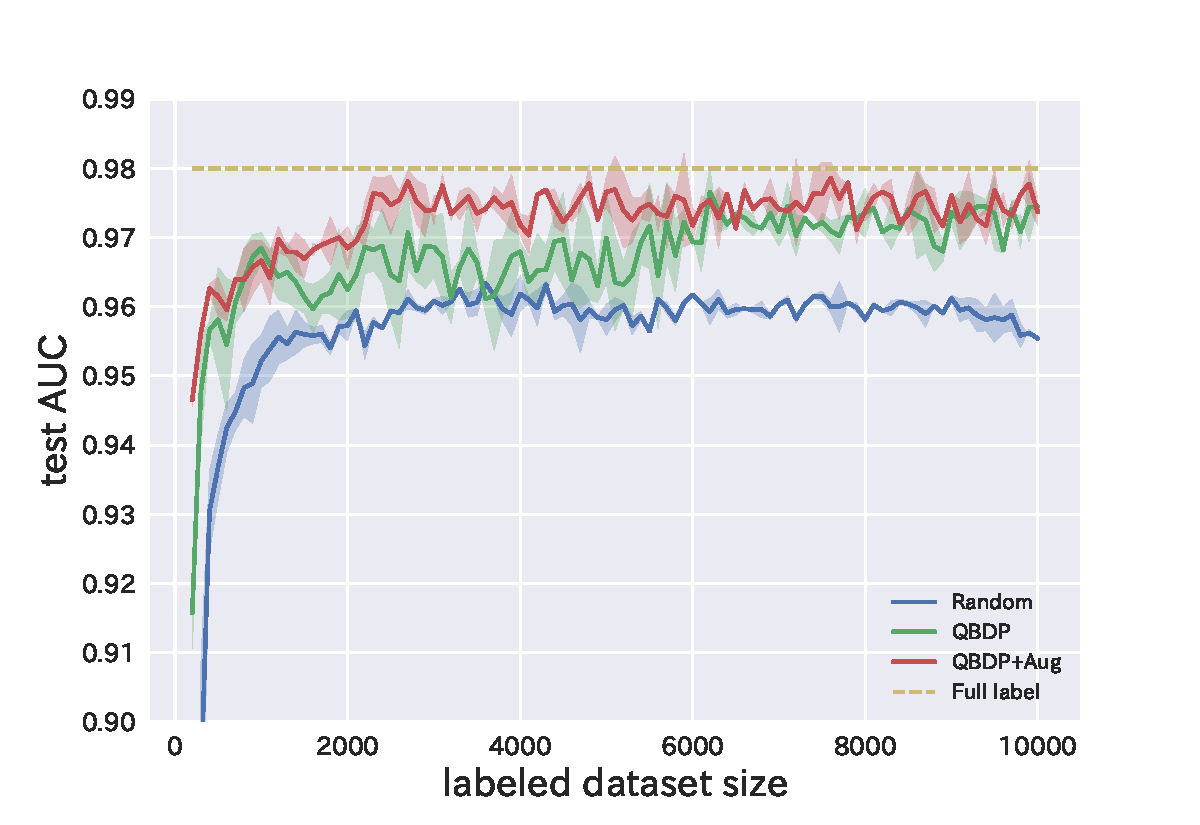
\includegraphics[width=12cm]{figures/camelyon_acc_graph.pdf}
     \end{center}
    \caption{各手法を利用した場合のラベル付きサンプル数の増加に対するテスト精度の変化を示した図}
\end{figure}

\begin{figure}[hbp]
  \begin{center}
      \subfloat[Random Sampling]{
        \scalebox{0.8}{
          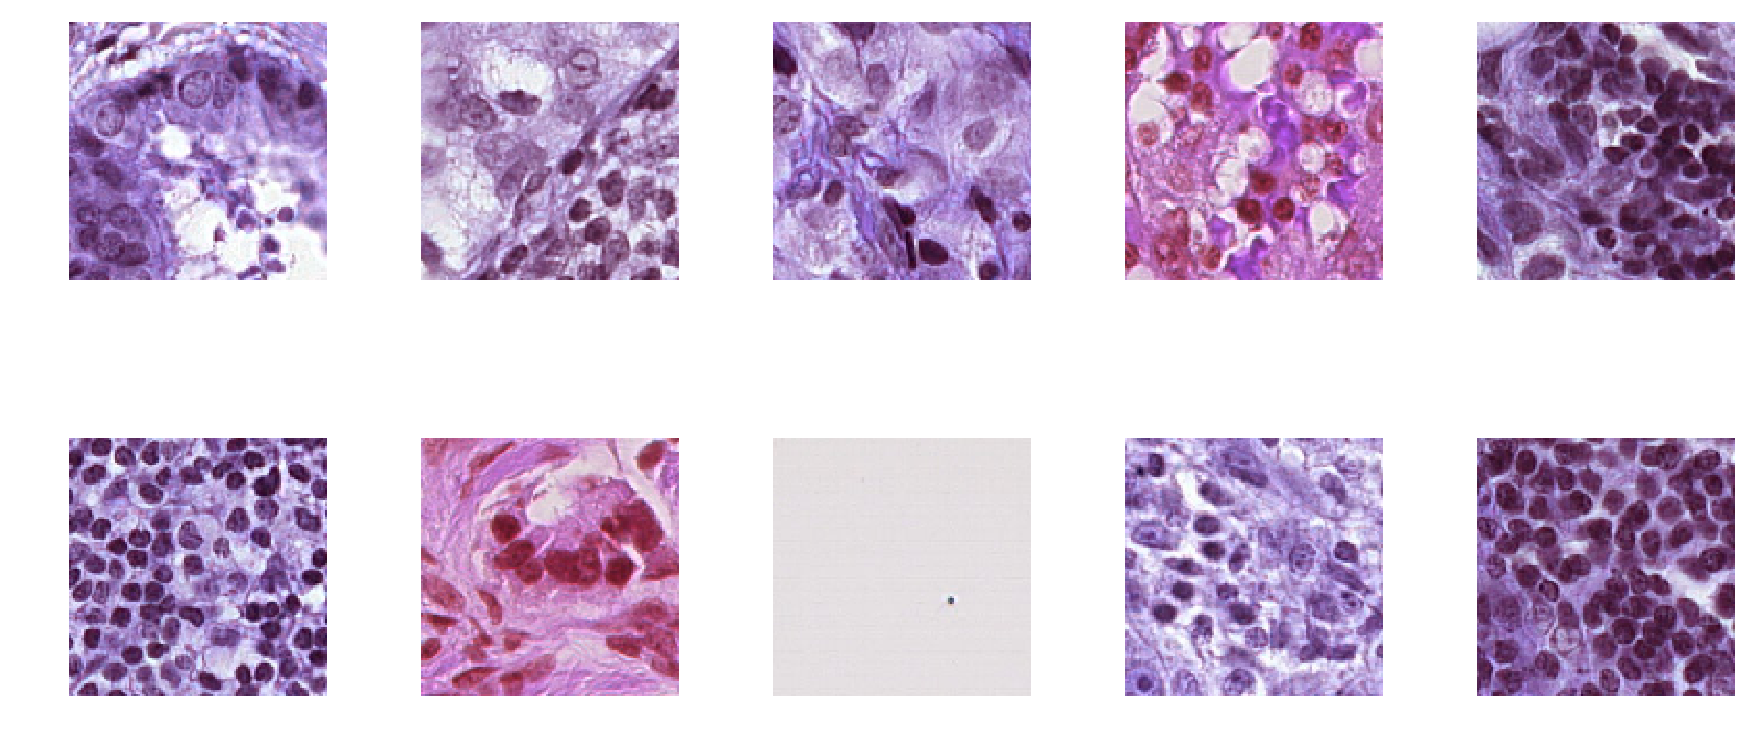
\includegraphics[width=8cm]{figures/camelyon_query_example_Random.pdf}
          }
      }

      \subfloat[Uncertain + QBDP]{
      \scalebox{0.8}{
          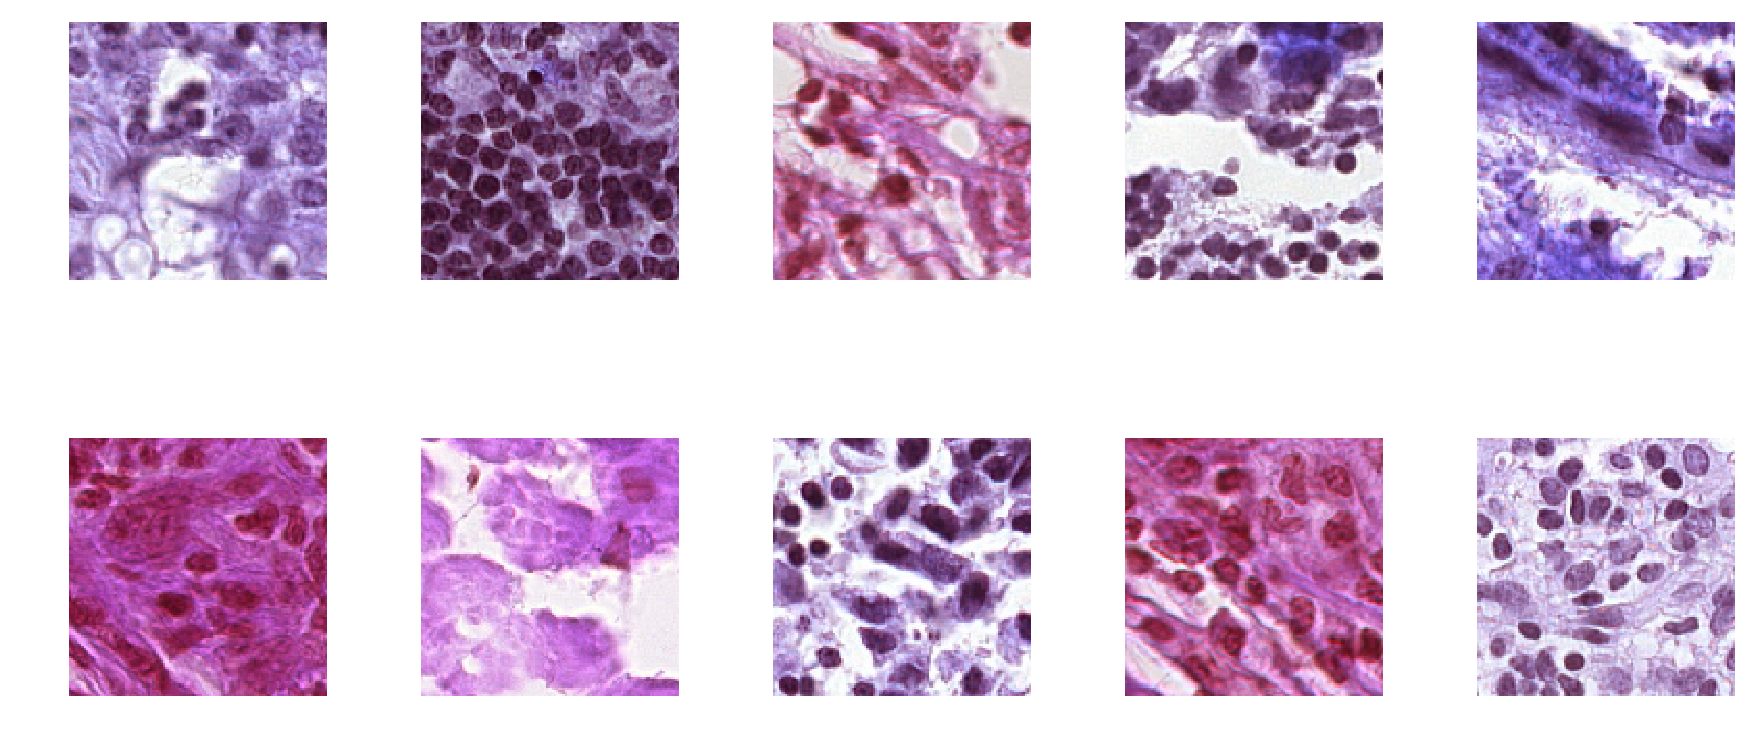
\includegraphics[width=8cm]{figures/camelyon_query_example_QBDP.pdf}
        }
      }
      \subfloat[Uncertain + QBDP + Aug]{
      \scalebox{0.8}{
      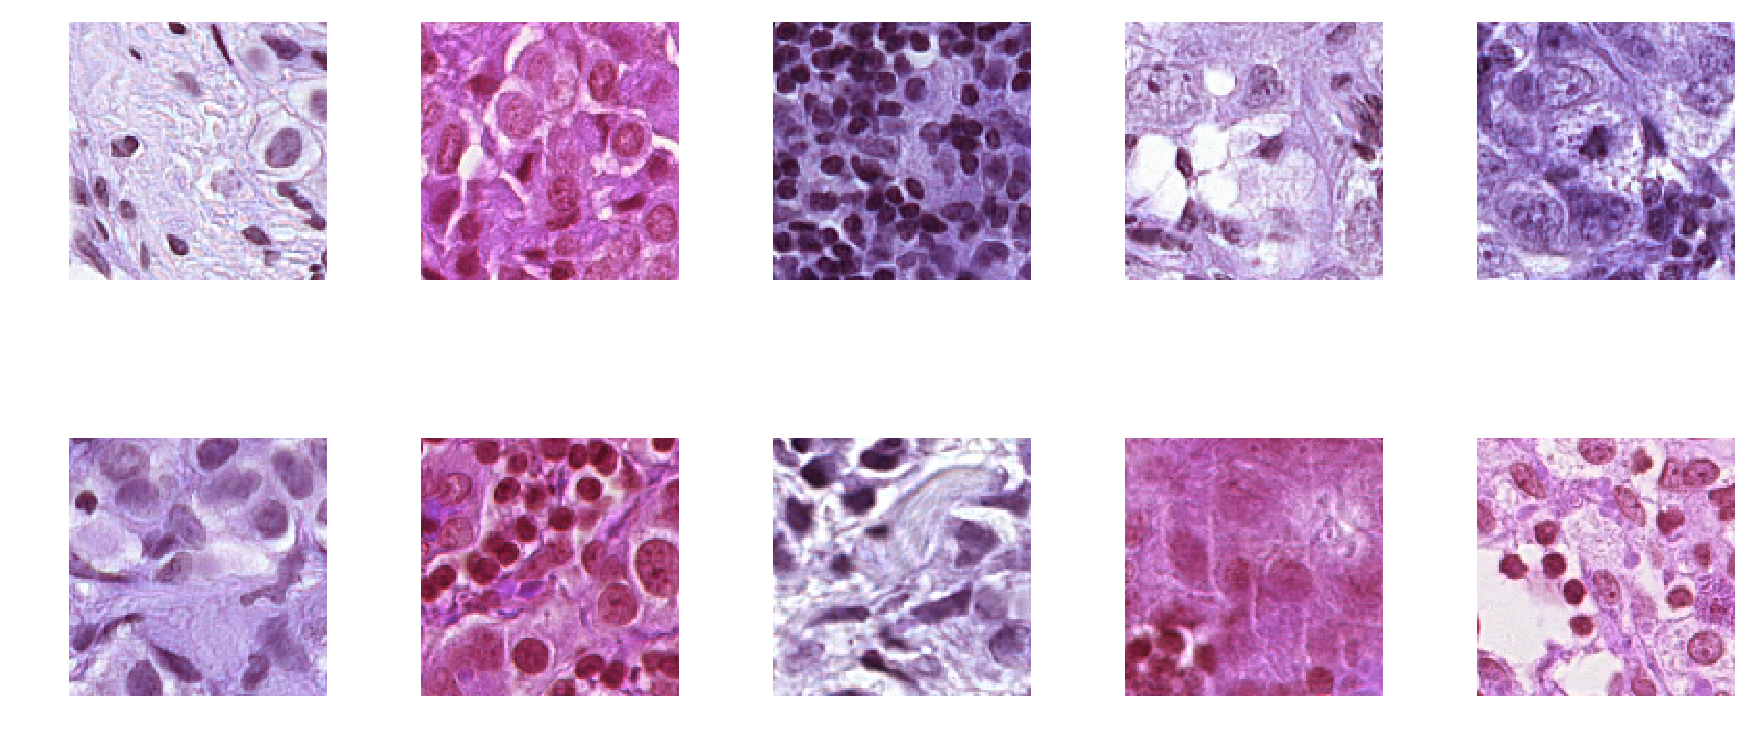
\includegraphics[width=8cm]{figures/camelyon_query_example_QBDP+Aug.pdf}
          }
      }
  \caption{\label{figure:camelyon_query_examples}各手法によってクエリとして選択されたサンプルを示す。}
  \end{center}
\end{figure}


\section{考察}
